\icode{E-MV-MU-L3-261011-001}
简谐横波在均匀介质中沿直线传播，\(P\)、\(Q\)是传播方向上相距\,\qty{10}{m}的两质点，波先传到\(P\)，当波传到\(Q\)开始计时，\(P\)、\(Q\)两质点的振动图象如图所示。则\paren[]

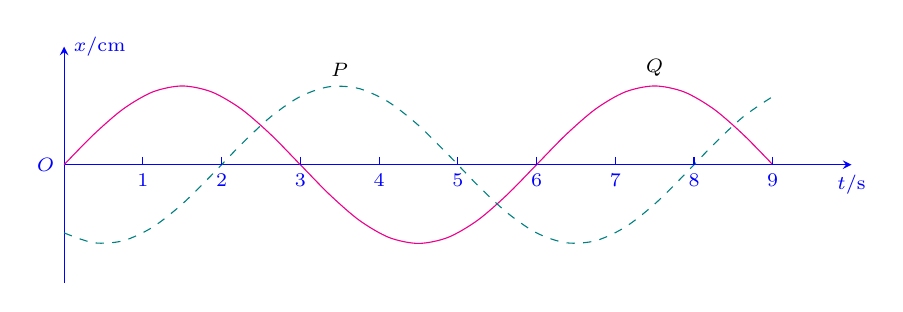
\begin{tikzpicture}[>=stealth,font=\scriptsize]
	\draw[->,blue] (0,-1.5)--(0,1.5)node[right]{\(x\)/\qty{}{cm}};
	\draw[->,blue] (0,0)node[left]{\(O\)}--(10,0)node[below]{\(t\)/\qty{}{s}};
	\draw[domain=0:9,smooth,magenta] plot(\x,{sin(pi*\x/3 r)});
	\draw[domain=0:9,smooth,dashed,teal] plot(\x,{sin((pi*\x/3-2*pi/3) r)});
	\foreach \x in {1,2,...,9}
		\draw[blue] (\x,.1)--(\x,0)node[below]{\(\x\)};
	\node at(7.5,1)[above]{\(Q\)};
	\node at(3.5,1)[above]{\(P\)};
\end{tikzpicture}
\begin{choices}
	\item 质点\(Q\)开始振动的方向沿\(y\)轴正方向
	\item 该波从\(P\)传到\(Q\)的时间可能为\qty{7}{s}
	\item 该波的传播速度可能为\qty{2}{m/s}
	\item 该波的波长可能为\qty{6}{m}
\end{choices}
\begin{answer}
    AD\qquad 提示：将\(P\)向右移动\(\frac{2}{3}T + nT\)（\(n = 0,1,3,\cdots\)），则\(\frac{2}{3}\lambda + n\lambda =\)\,\qty{10}{m}，\(\lambda = \frac{30}{3n + 2}\)（\(n = 0,1,3,\cdots\)）
\end{answer}